W czasie ładowania się systemu operacyjnego będzie widoczne logo Ubuntu ze stopniowo wypełniającymi się kwardratami. Wciskając dowolny klawisz logo zostanie zastąpione szczególowym opisem tego co jest aktualnie wykonywane.

Kiedy proces uruchamiania systemu dobiegnie końca twoim oczom ukarze się ekran logowania systemu Ubuntu (jeżeli w czasie instalacji wybrałeś "Automatyczne Logowanie" to ten ekran zostanie pominięty i automatycznie zostaniesz przeniesiony do pulpitu).
\begin{center}
	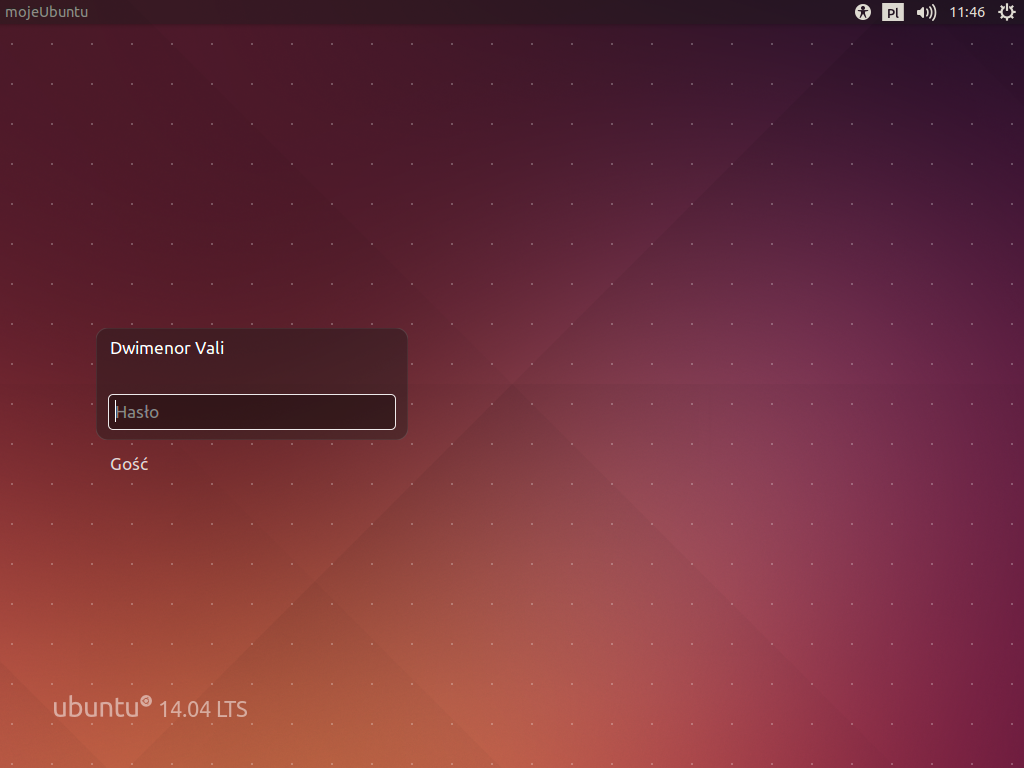
\includegraphics[scale=0.5]{images/greater.png}
\end{center}

\begin{enumerate}
\item Lista użytkowników systemu. Jeżeli w systemie jest więcej niż jeden użytkownik to z tej listy będzie można wybrać kto ma zostać zalogowany.
\item W to pole wpisz hasło aktualnie wybranego użytkownika.
\item Konto gość umozliwia zalogowanie się do systemu bez podawania hasła. Wszystkie zmiany wprowadzone przez gościa (np. utworzone pliki) zostaną utracone po zakończeniu sesji.
\item Nazwa systemu wybrana podczas instalacji.
\item Przyciski sterujące
\begin{description}
\item[
\includegraphics{images/ikony_dostempnosc2.png}]Dostepność - uruchomienie lupy, czytnika ekranowego lub klawiatury ekranowej.
\item[
\includegraphics{images/ikony_jezyk.png}]Język - pozwala zmienić układ klawiatury i metodę wprowadzania tekstu.
\item[
\includegraphics{images/ikony_dzwiek.png}]Ustawienia głośności i dźwięku.
\item[\textbf{11:46}] Zegar i kalendarz.
\item[
\includegraphics{images/ikony_zasilanie.png}]Wyłączenie lub ponowne uruchomienie komputera.
\end{description}
\end{enumerate}
\clearpage